
\subsection{PB}
\subsubsection{Primo Incremento}

\paragraph{Consuntivo Orario}
\begin{center}
	\renewcommand{\arraystretch}{1.8} %aumento ampiezza righe
	\begin{tabular}{ |m{8em}|c|c|c|c|c|c|c| }
	\hline
	\textbf{Membro} & \textbf{Re} & \textbf{Am} &  \textbf{An} &  \textbf{Pt} &  \textbf{Pg} &  \textbf{Ve} &  \textbf{Totale}\\
    \hline
    Irene Benetazzo   & - & 1 (+1)  & 3 (+3)  & 5 (-3)  & 5       & 4 (+1)  & \textbf{18} (+2) \\
    \hline
    Tommaso Berlaffa  & 3 & -       & 1 (+1)  & -       & 8 (-2)  & 1 (+1)  & \textbf{13} \\
    \hline
    Mattia Episcopo   & - & 3 (-1)  & 2 (+2)  & 7       & 4       & 2       & \textbf{18} (+1) \\
    \hline
    Pietro Macrì      & - & - (-4)  & -       & 6 (+1)  & 6 (-1)  & 2       & \textbf{14} (-4)\\
    \hline
    Qi Fan Andrea Pan & - & -       & -       & 8 (+1)  & 6 (-1)  & 2  (-1) & \textbf{16} (-1) \\
    \hline
    Matteo Pillon     & - & -       & -       & 6 (+1)  & 6 (-2)  & 2  (-1) & \textbf{14} (-2) \\
    \hline
    Samuele Rizzato   & - & 2 (+2)  & 2 (+2)  & 6 (-2)  & 5       & 2  (-1) & \textbf{17} (+1) \\
    \hline
    \textbf{Totale ore} & \textbf{3} & \textbf{8} & \textbf{8} (+8) &  \textbf{38} (-2) &  \textbf{40} (-6) &  \textbf{15} (-1) &  \textbf{110} (-3)\\
    \hline
	\end{tabular}
\end{center}
\begin{figure}[H]
    \centering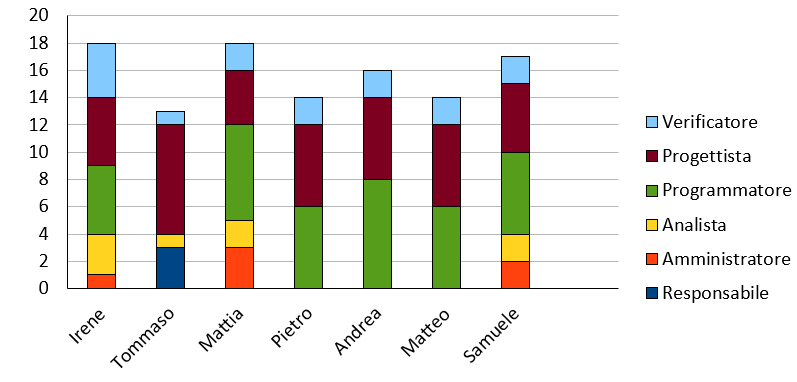
\includegraphics[width=\textwidth, height=\textheight,keepaspectratio]{images/consuntivo/PB-ore.png}
    \caption{PB - Product Baseline - Primo Incremento - consuntivo ripartizione oraria}
\end{figure}

\paragraph{Consuntivo Economico}
\begin{center}
	\renewcommand{\arraystretch}{1.8}
	\begin{tabular}{ |m{6em}|c|c|c|c|c|c|c| }
	\hline
	\textbf{Ruolo} & \textbf{Re} & \textbf{Am} &  \textbf{An} &  \textbf{Pt} &  \textbf{Pg} &  \textbf{Ve} &  \textbf{Totale}\\
    \hline
    Totale ore & 3 & 8 & 8 & 38 & 40 & 14 & \textbf{110}\\
    \hline
    Costo \euro/h & 30\euro/h & 20\euro/h & 25\euro/h & 25\euro/h & 15\euro/h & 15\euro/h & \\
    \hline
    \textbf{Totale costo} & \textbf{90\euro} & \textbf{120\euro} &  \textbf{200\euro} & \textbf{950\euro} &  \textbf{600\euro} &  \textbf{225\euro} &  \textbf{2185\euro} \\
    &  & (-40\euro) & (+200\euro) & (-50\euro) & (-90\euro) & (-25\euro) & (+5\euro) \\
    \hline
	\end{tabular}

    \begin{figure}[H]
        \centering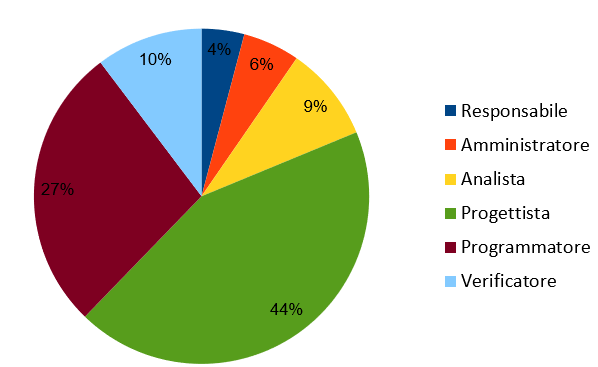
\includegraphics[width=0.7\textwidth, height=0.7\textheight, keepaspectratio]{images/consuntivo/PB-costo.png}
        \caption{PB - Product Baseline - Primo Incremento - consuntivo ripartizione economica}
    \end{figure}
\end{center}

\paragraph{Considerazioni} \hfill \break
L'inizio della fase è stato posticipato, causa revisione con i docenti. A seguito di quest'ultima, 
sono state necessarie ulteriori ore di analista per gestire la correzione e l'analisi di possibili soluzioni della documentazione presentata durante colloquio.\\
L'intera fase di Product Baseline viene quindi temporalmente traslata di conseguenza.

\begin{center}
	\renewcommand{\arraystretch}{1.8}
	\begin{tabular}{ | l |c|c| }
    \hline
    & \textbf{Ore} & \textbf{Costo} \\
	\hline
    \textbf{Consuntivo} & 110 & 2185\euro \\
    \hline
    \textbf{Preventivo} & 113 & 2180\euro \\
    \hline
    \textbf{Bilancio fase} & -3 & -5\euro \\
    \hline
    \textbf{Bilancio complessivo} & \textbf{-39} & \textbf{-890\euro} \\
    \hline
    \end{tabular}
\end{center}
In conclusione il primo incremento della fase Product Baseline termina il 2022-07-20 con un risparmio, relativo
alla fase, di 5€.

\newpage

\subsubsection{Secondo Incremento}

\paragraph{Consuntivo Orario}
\begin{center}
	\renewcommand{\arraystretch}{1.8} %aumento ampiezza righe
	\begin{tabular}{ |m{8em}|c|c|c|c|c|c|c| }
	\hline
	\textbf{Membro} & \textbf{Re} & \textbf{Am} &  \textbf{An} &  \textbf{Pt} &  \textbf{Pg} &  \textbf{Ve} &  \textbf{Totale}\\
    \hline
    Irene Benetazzo   & - & -  & -  & 7  & 5 & 2 (-1) & \textbf{14} \\
    \hline
    Tommaso Berlaffa  & - & - & -  & 6 & 6  & 2 (-1) & \textbf{14} \\
    \hline
    Mattia Episcopo   & 3 & -  & -  & - & 10 & 0 & \textbf{13} \\
    \hline
    Pietro Macrì      & - & -  & - & 5 & 6 & 2 (-1) & \textbf{13} \\
    \hline
    Qi Fan Andrea Pan & - & 2 (-2) & - & 4 & 8 & 2 (-1) & \textbf{16} \\
    \hline
    Matteo Pillon     & - & - & - & 6 & 7 & 2 (-1) & \textbf{15} \\
    \hline
    Samuele Rizzato   & - & 3 (-2) & - & 6 & 5 & 2 (-1) & \textbf{16} \\
    \hline
    \textbf{Totale ore} & \textbf{3} & \textbf{5} (-4) & \textbf{0} &  \textbf{34} &  \textbf{47} &  \textbf{12} (-5) &  \textbf{101} (-9)\\
    \hline
	\end{tabular}
\end{center}
\begin{figure}[H]
    \centering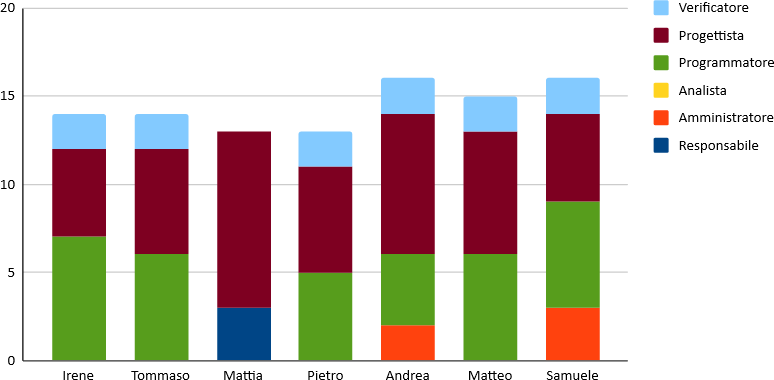
\includegraphics[width=\textwidth, height=\textheight,keepaspectratio]{images/consuntivo/consuntivo-PB-ore-secondo-incremento.png}
    \caption{PB - Product Baseline - Secondo Incremento - consuntivo ripartizione oraria}
\end{figure}

\paragraph{Consuntivo Economico}
\begin{center}
	\renewcommand{\arraystretch}{1.8}
	\begin{tabular}{ |m{6em}|c|c|c|c|c|c|c| }
	\hline
	\textbf{Ruolo} & \textbf{Re} & \textbf{Am} &  \textbf{An} &  \textbf{Pt} &  \textbf{Pg} &  \textbf{Ve} &  \textbf{Totale}\\
    \hline
    Totale ore & 3 & 5 & 0 & 34 & 47 & 12 & \textbf{101}\\
    \hline
    Costo \euro/h & 30\euro/h & 20\euro/h & 25\euro/h & 25\euro/h & 15\euro/h & 15\euro/h & \\
    \hline
    \textbf{Totale costo} & \textbf{90\euro} & \textbf{100\euro} &  \textbf{0\euro} & \textbf{850\euro} &  \textbf{705\euro} &  \textbf{180\euro} &  \textbf{1925\euro} \\
    &  & (-80\euro) & & & & (-75\euro) & (-155\euro) \\
    \hline
	\end{tabular}

    \begin{figure}[H]
        \centering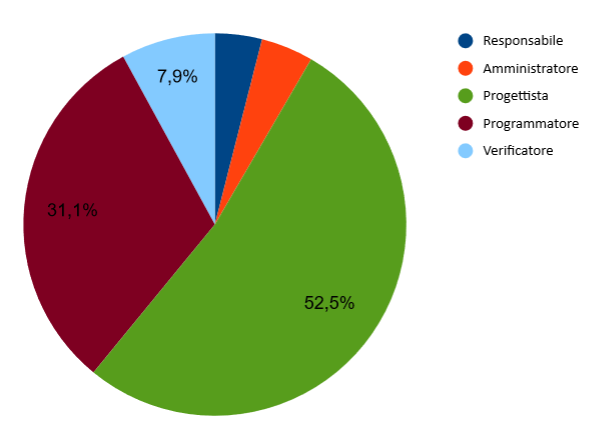
\includegraphics[width=0.7\textwidth, height=0.7\textheight, keepaspectratio]{images/consuntivo/consuntivo-PB-costo-secondo-incremento.png}
        \caption{PB - Product Baseline - Secondo Incremento - consuntivo ripartizione economica}
    \end{figure}
\end{center}

\paragraph{Considerazioni} \hfill \break
Il secondo incremento era stato sovrastimato in sede di preventivo, sia come ore che come costi. In termini di ore c'è stato un discreto risparmio di tempo per i ruoli di verificatore (4) e amministratore (5) che hanno portato ad un risparmio complessivo di 9 ore.
\begin{center}
	\renewcommand{\arraystretch}{1.8}
	\begin{tabular}{ | l |c|c| }
    \hline
    & \textbf{Ore} & \textbf{Costo} \\
	\hline
    \textbf{Consuntivo} & 101 & 1925\euro \\
    \hline
    \textbf{Preventivo} & 110 & 2080\euro \\
    \hline
    \textbf{Bilancio fase} & -9 & -155\euro \\
    \hline
    \textbf{Bilancio complessivo} & \textbf{-48} & \textbf{-1045\euro} \\
    \hline
    \end{tabular}
\end{center}
In conclusione il secondo incremento della fase Product Baseline termina il 2022-08-03 con un risparmio economico, relativo alla fase, di 155€.

